\documentclass[../../tesis_maestria]{subfiles}
\begin{document}

\chapter{El dominio fundamental de $\Gamma_0(15)$}
La siguente imagen es el dominio fundamental de la acci\'on $\Gamma_0(15)\act\HH$:

\begin{figure}[!h]%%%%%%%%%%%%%%%%%%%%%%%%%%%%%%%%%%%%%%%%%%%% FIGURA
  \centering
  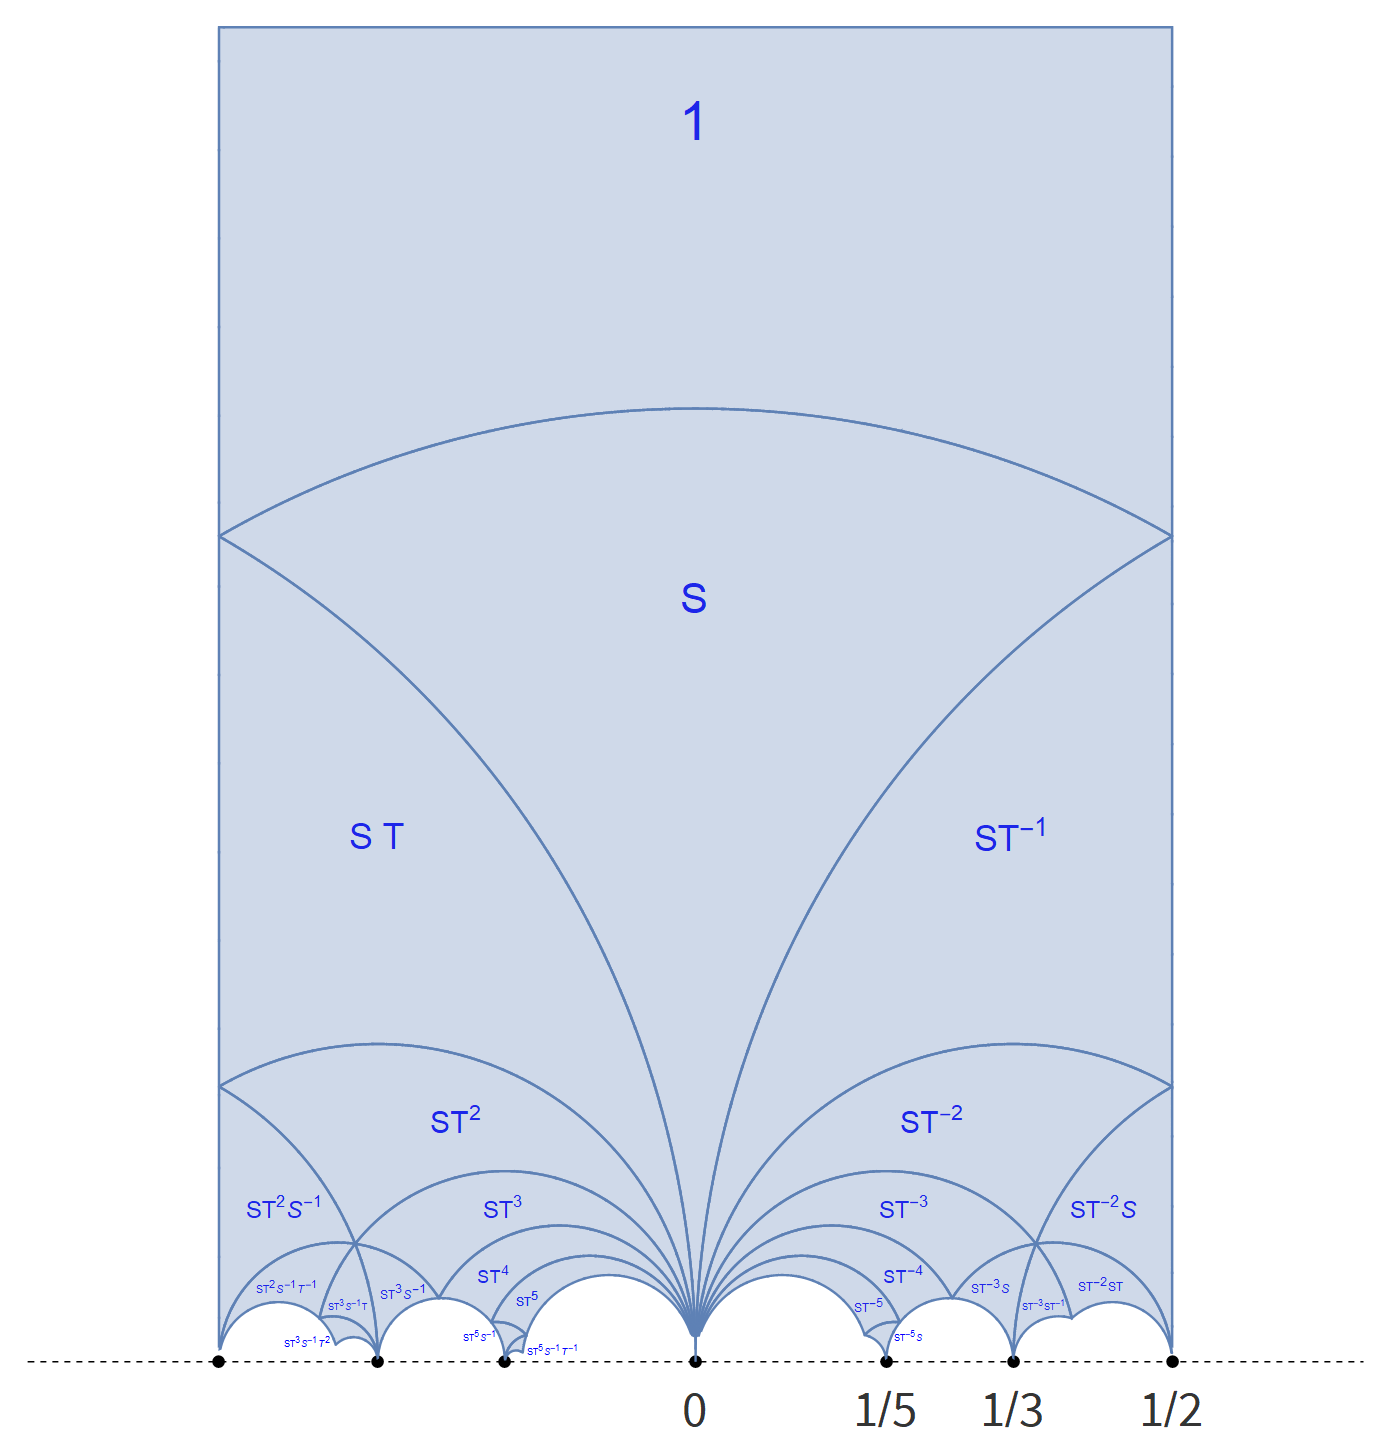
\includegraphics[scale=0.3]{domfundgamma015labeled}
%  \label{fig:topologiaH}
\end{figure}%%%%%%%%%%%%%%%%%%%%%%%%%%%%%%%%%%%%%%%%%%%%%%%%%%%%%%%%%%%%%%%%%%%%%%%%%%

%Cada secci\'on del dominio fundamental viene etiquetada con la matriz que traslada el dominio
%fundamental de $\SL_2(\ZZ)$ a la secci\'on correspondiente. Aqu\'i la notaci\'on es:
%\[
%  T=\mat{1}{1}{0}{1}\qquad\text{y}\qquad S=\mat{0}{1}{-1}{0}.
%\]

\section{Una transformada de Fourier}

El prop\'osito de este ap\'endice es estudiar la transformada de Fourier de la funci\'on $\phi$
que aparece en la secci\'on \ref{sec:formas_modulares} y que est\'a definido por:
\[
  \phi_{y,s}(x):=\phi(x+iy;s)=\frac{1}{(x+iy)^{1+s}(x-iy)^s}.
\]
M\'as precisamente queremos probar la siguiente proposici\'on:

\begin{prop}\label{ap:de_phihat}
  Sean $y>0$ y $t\neq0$ fijos y denota $\varphi_{y,t}(s):=\hat{\phi}_{y,s}(t)$. Entonces:
  \begin{enumerate}[label=\roman*)]
  \item $\varphi_{y,t}(s)$ es holomorfa en el semiplano $\HH'$.
  \item $\varphi_{y,t}(s)$ admite una extensi\'on holomorfa a todo $\CC$ definida por
    \begin{equation}\label{ap:formulaphihat}
      \varphi_{y,t}(s)=\hat{\phi}_{y,s}(t)=
      \begin{cases}
        \dfrac{i\pi^st^{s-1}e^{-2\pi ty}}{2\Gamma(s)y^{s+1}}\st(4\pi ty;s,s+1) &t>0\\
        2\pi i(2y)^{-2s}\Gamma(2s)\Gamma(s)^{-1}\Gamma(s+1)^{-1} &t=0\\
        \dfrac{2i\pi^{s+1}|t|^se^{-2\pi|t|y}}{y^s\Gamma(s+1)}\st(4\pi|t|y;s+1,s) &t<0
      \end{cases}.
    \end{equation}
    donde
    \[
      \st(z;\alpha,\beta):=\frac{z^{\beta}}{\Gamma(\beta)}\int_0^{\infty}e^{-zw}(w+1)^{\alpha-1}w^{\beta-1}dw
  \qquad(\Re(z),\Re(\beta)>0,\alpha\in\CC).
    \]
  \item\label{ap:inciso3} En particular:
    \[
      \varphi_{y,t}(0)=\hat{\phi}_{y,0}(t)=
      \begin{cases}
        0 & t>0\\
        2\pi i e^{2\pi ty} &t<0
      \end{cases}
    \]
  \item\label{ap:inciso4} Para todo subconjunto compacto $Q\subset\CC$ existen constantes $A,B>0$
    tales que
    \[
      |\varphi_{y,t}(s)|=|\hat{\phi}_{y,s}(t)|\leq
      \begin{cases}
        A y^{-\Re(s)-1}t^{\Re(s)-1}(1+(4\pi yt)^{-B})e^{-2\pi yt} & t>0\\
        A y^{-\Re(s)}|t|^{\Re(s)}(1+(4\pi |t|y)^{-B})e^{-2\pi|t|y} & t<0
      \end{cases}
    \]
  \end{enumerate}
\end{prop}

En \eqref{eq:approxdephi} de la secci\'on \ref{sec:eisenstein} vimos que para $y>0$ y para
$\Re(s)>0$ tenemos que $\phi_{y,s}$ es absolutamente integrable y admite una transformada de Fourier:
\begin{equation}
  \label{ap:phihat}
  \hat{\phi}_{y,s}(t)=\int_{-\infty}^{\infty}\phi_{y,s}(x)e^{-2\pi i tx}dx
  \qquad \big(y>0,\; \Re(s)>0\big).
\end{equation}
De esta manera podemos calcular $\hat{\phi}$ con el siguiente lema t\'ecnico:

\begin{lema}%%%%%%%%%%%%%%%%%%%%%%%%%%%%%%%%%%%%%%%%%%%%%%%%%%%%%%%%%%%%%%%%%%%%%%%%%%% THEOREMA
  Para $y>0$ y $\Re(s)>0$ fijas, tenemos la siguiente f\'ormula:
  \begin{equation}\label{eq:trans_de_phi}
  \hat{\phi}_{y,s}(t)=
  \begin{cases}
    2\pi i(2\pi t)^{2s}e^{-2\pi yt}\Gamma(s)^{-1}\Gamma(s+1)^{-1}\sigma(4\pi yt;s,s+1) &\;\;(t>0)\\
    2\pi i\Gamma(2s)(2y)^{-2s}\Gamma(s)^{-1}\Gamma(s+1)^{-1} &\;\; (t=0)\\
    2\pi i(2\pi t)^{2s}e^{-2\pi y\abs{t}}\Gamma(s)^{-1}\Gamma(s+1)^{-1}\sigma(4\pi y\abs{t};s+1,s)%
    &\;\;(t<0)
  \end{cases} 
\end{equation}
donde
\[
  \sigma(z;\alpha,\beta)=\int_0^{\infty}e^{-zw}(w+1)^{\alpha-1}w^{\beta-1}dw
  \qquad(\Re(z),\Re(\beta)>0,\alpha\in\CC),
\]
es una representaci\'on integral de la \emph{funci\'on hipergeom\'etrica confluente}
(cf. \ref{ap:fun_hipergeo_conf})
\end{lema}%%%%%%%%%%%%%%%%%%%%%%%%%%%%%%%%%%%%%%%%%%%%%%%%%%%%%%%%%%%%%%%%%%%%%%%%%%%%%%%%%%%%%%%%%

\begin{proof}
  Para calcular la integral \eqref{ap:phihat}, hay que
  expresar los dos factores del denominador, como transformadas de Fourier de otras funciones. Primero
  reescribimos el integrando:
\[
  (x+iy)^s(x-iy)^{s+1}=
  (i(y-ix))^s(-i(y+ix))^{s+1}\overset{*}{=}
  -i(y-ix)^s(y+ix)^{s+1},
\]
donde (*) es v\'alido porque $\Re(y\pm ix)>0$, entonces:
\begin{equation}\label{eq:trans_de_phii}
  \hat{\phi}_{y,s}(t)=
  i\int_{-\infty}^{\infty}\frac{e^{-2\pi itx}dx}{(y-ix)^s(y+ix)^{s+1}}.
\end{equation}

Ahora estudiamos los factores del denominador de \eqref{eq:trans_de_phii}. Para esto, definimos:
\[
  f_{\pm}(x):=\frac{1}{(y\pm ix)^{s+1}} \qquad,\qquad
  g(w):=
  \begin{cases}
    e^{-yw}w^s &(0<w)\\
    0 &(w\leq 0)
  \end{cases}
\]
donde $g(w)$ es absolutamente integrable porque $y>0$ y $\Re(s)>0$. Si calculamos su transformada de
Fourier, obtenemos:
\begin{gather}
  \hat{g}\paren{\frac{\pm x}{2\pi}}=
  \int_{-\infty}^{\infty}e^{\mp iwx}g(w)dw=
  \int_0^{\infty}e^{-(y\pm ix)w}w^sdw\overset{*}{=}
  (y\pm ix)^{-s-1}\Gamma(s+1),\nonumber\\
  \therefore \quad f_{\pm}(x)=\frac{1}{\Gamma(s+1)} \hat{g}\paren{\frac{\pm x}{2\pi}}
  \label{eq:trans_de_g_dos}
\end{gather}
donde el paso (*) se sigue de que la funci\'on gamma cumple
\begin{gather}
  \int_0^{\infty}e^{-zt}t^{v-1}dt=
  \int_0^{\infty}e^{-z'}\paren{\tfrac{z'}{z}}^{v-1}\frac{dz'}{z}=
  z^{-v}\int_0^{\infty}e^{-z'}(z')^{v-1}dz'\nonumber\\
  \therefore\;\;z^{-v}\Gamma(v) = \int_0^{\infty}e^{-zt}t^{v-1}dt
  \qquad(\Re(z),\Re(v)>0)\label{eq:prop_gamma}
\end{gather}
(por ejemplo \cite[\S5.2.5]{AhlforsCA}). En general y de manera similar, tenemos:
\begin{equation}\label{eq:denominador}
  \frac{1}{(y\pm ix)^s}=
  \frac{1}{\Gamma(s)}\int_0^{\infty}e^{-(y\pm ix)w}w^{s-1}dw\qquad(\Re(s)>0)
\end{equation}
Si aplicamos la transformada de Fourier a \eqref{eq:trans_de_g_dos} obtenemos
\begin{equation}\label{eq:trans_de_f}
  \int_{-\infty}^{\infty}\frac{e^{-2\pi iwx}dx}{(y\pm ix)^{s+1}}=\hat{f}_{\pm}(w)=
  \frac{2\pi}{\Gamma(s+1)}g\paren{\mp 2\pi w}
\end{equation}
donde hemos usado la f\'ormula de inversi\'on de Fourier, i.e. $\hat{\hat{g}}(x)=g(-x)$ y c\'omo
cambia la transformada de Fourier bajo homotecias, i.e.
$\widehat{g(\delta w)}(x)=\delta^{-1}g(\delta^{-1}x)$. Con estas funciones auxiliares podemos
calcular \eqref{eq:trans_de_phii}.

Sustituimos la f\'ormula \eqref{eq:denominador} en \eqref{eq:trans_de_phii} para obtener:
\begin{equation}\label{eq:phidobleint}
  \hat{\phi}_{y,s}(t)=
  \frac{i}{\Gamma(s)}\int_{-\infty}^{\infty}\frac{e^{-2\pi itx}}{(y+ix)^{s+1}}
  \paren{\int_0^{\infty}e^{-(y-ix)w}w^{s-1}dw}dx.
\end{equation}
Ahora aproximamos el integrando:
\[
  \abs{\frac{e^{-2\pi itx}}{(y+ix)^{s+1}}e^{-(y-ix)w}w^{s-1}}
  =\abs{x+iy}^{-\Re(s)-1}e^{-yw}w^{\Re(s)-1}=
  \begin{cases}
    O(\abs{x}^{-\Re(s)-1}) & x\ra\pm\infty\\
    O(w^{\Re(s)-1}) & w\ra 0\\
    O(e^{-yw}) & w\rai
  \end{cases}.
\]
Esto implica que bajo las hip\'otesis $y>0$ y $\Re(s)>0$, la doble integral \eqref{eq:phidobleint}
es absolutamente integrable. Por el teorema de Fubini\footnote{Teorema y Cita...}
podemos intercambiar el orden de integraci\'on para obtener:
\begin{align}
  \hat{\phi}_{y,s}(t)&=
  \frac{i}{\Gamma(s)}\int_{0}^{\infty}w^{s-1}e^{-yw}
  \paren{\int_{-\infty}^{\infty}
  \frac{e^{-2\pi ix\paren{t-\tfrac{w}{2\pi}}}}{(y+ix)^{s+1}}dx}dw\nonumber\\
  &\overset{\eqref{eq:trans_de_f}}{=}\frac{i}{\Gamma(s)}\int_{0}^{\infty}w^{s-1}e^{-yw}
    \paren{\frac{2\pi}{\Gamma(s+1)}g\paren{w-2\pi t}}dw\nonumber\\
  &=\frac{2\pi i}{\Gamma(s)\Gamma(s+1)}
    \int_{2\pi t}^{\infty}e^{-2y(w-\pi t)}w^{s-1}(w-2\pi t)^sdw\nonumber\\
   &=\frac{2\pi i}{\Gamma(s)\Gamma(s+1)}\int_{\pi t}^{\infty}e^{-2yw}(w+\pi t)^{s-1}(w-\pi t)^sdw,
   \label{eq:phisemifinal}
\end{align}
donde la \'ultima igualdad se deriva con el cambio de variable $w-\pi t\mapsto w$. Esta \'ultima
f\'ormula es donde nuestros c\'alculos divergen seg\'un el valor de $t$.

Si $t=0$ aplicamos la ecuaci\'on \eqref{eq:prop_gamma}:
\[
  \hat{\phi}_{y,s}(0)=\frac{2\pi i}{\Gamma(s)\Gamma(s+1)}\int_0^{\infty}e^{-2yu}u^{2s-1}du=
  \frac{2\pi i\Gamma(2s)}{(2y)^{2s}\Gamma(s)\Gamma(s+1)}.
\]

Si $t\neq0$ consideramos ambos signos de $t$ en el mismo c\'alculo escibiendo $t=\pm|t|$. En la
integral \eqref{eq:phisemifinal} hacemos dos cambios de variable: $w\mapsto\pi |t| w$ y luego
$w\mapsto w+1$.
\begin{align}
  \hat{\phi}_{y,s}(t)&=
  \frac{2\pi i}{\Gamma(s)\Gamma(s+1)}
  \int_1^{\infty}e^{-2\pi y|t|w}(\pi|t|w+\pi t)^{s-1}(\pi w|t|-\pi t)^s(\pi |t|)dw\nonumber\\
  &=\frac{2\pi i(\pi |t|)^{2s}}{\Gamma(s)\Gamma(s+1)}
  \int_1^{\infty}e^{-2\pi y|t|w}(w\pm1)^{s-1}(w\mp 1)^sdw\nonumber\\
  &=\frac{2\pi i(\pi |t|)^{2s}e^{-2\pi y|t|}}{\Gamma(s)\Gamma(s+1)}
    \underset{I_{\pm}}{\underbrace{\int_0^{\infty}e^{-2\pi y|t|w}(w\pm1+1)^{s-1}(w\mp1+1)^sdw}}\nonumber\\
%  &=\frac{2\pi i(2\pi t)^{2s}e^{-2\pi yt}}{\Gamma(s)\Gamma(s+1)}
%    \int_0^{\infty}e^{-4\pi ytw}(w+1)^{s-1}w^sdw\qquad(t>0).\label{eq:u_posi}
\end{align}
Ahora calculamos la integrales $I_{\pm}$ por separado. En ambos c\'alculos hacemos el cambio de
variable $w\mapsto 2w$. Primero asumimos que $t>0$, entonces
\begin{align*}
  I_+
  &=\int_0^{\infty}e^{-2\pi ytw}(w+2)^{s-1}w^sdw=2^{2s}\int_0^{\infty}e^{-4\pi ytw}(w+1)^{s-1}w^sdw
    \qquad(t>0)\\
  \therefore\quad\hat{\phi}_{y,s}(t)
  &=\frac{2\pi i(\pi t)^{2s}e^{-2\pi yt}}{\Gamma(s)\Gamma(s+1)}\sigma(4\pi ty;s,s+1)\qquad(t>0)
\end{align*}
donde $\sigma$ es la (f\'ormula integral de la) \emph{funci\'on hipergeom\'etrica confluente} definida
como:
\[
  \sigma(z;\alpha,\beta)=\int_0^{\infty}e^{-zw}(w+1)^{\alpha-1}w^{\beta-1}dw
  \qquad(\Re(z),\Re(\beta)>0,\alpha\in\CC).
\]
Ahora asumimos que $t<0$ y similarmente tenemos:
\begin{align*}
  I_{-}
  &=\int_0^{\infty}e^{-2\pi|t|yw}w^{s-1}(w+2)^sdw=2^{2s}\int_0^{\infty}e^{-4\pi|t|yw}(w+1)^sw^{s-1}dw
    \qquad(t<0)\\
  \therefore\quad\hat{\phi}_{y,s}(t)
  &=\frac{2\pi i(\pi |t|)^{2s}e^{-2\pi y|t|}}{\Gamma(s)\Gamma(s+1)}\sigma(4\pi|t|y;s+1,s)\qquad(t<0).
\end{align*}
Con esto terminamos de verificar la f\'ormula \eqref{eq:trans_de_phi}.
\end{proof}

Ahora enunciamos unas propiedades de la funci\'on hipergeom\'etrica confluente, propadas en
los teoremas 7.2.4 y 7.2.7 de \S 7.2 de \cite{MiyakeMF} o en el ap\'endice
\ref{ap:fun_hipergeo_conf}.

\begin{prop}\label{ap:prop_de_sigma}%%%%%%%%%%%%%%%%%%%%%%%%%%%%%%%%%%%%%%%%%%%%%%%%%%%%%%% TEOREMA
  La funci\'on $\sigma(z;\alpha,\beta)$ admite una continuaci\'on meromorfa a $\HH'\times\CC\times\CC$
  con polos cuando $\beta=0,-1,-2,\ldots$. En particular la funci\'on:
  \[
    \st(z;\alpha,\beta):=\frac{z^{\beta}}{\Gamma(\beta)}\sigma(z;\alpha,\beta)
  \]
  es una funci\'on holomorfa sobre $\HH'\times\CC\times\CC$ y para cualquier compacto
  $Q\subset\CC\times\CC$ y $y>0$ fija, existen constantes $A,B>0$ tales que
  \[
    |\st(y;\alpha,\beta)|\leq A(1+y^{-B}).
  \]
\end{prop}%%%%%%%%%%%%%%%%%%%%%%%%%%%%%%%%%%%%%%%%%%%%%%%%%%%%%%%%%%%%%%%%%%%%%%%%%%%%%%%%%%%%%%%%%%

En vista de la proposici\'on anterior, reescibimos $\hat{\phi}_{y,s}(t)$ en t\'erminos de $\st$ para
aproximar $|\hat{\phi}_{y,s}|$. Cuando $t>0$ tenemos que:
\begin{align}
  \hat{\phi}_{y,s}(t)
  &=\frac{2\pi i(2\pi t)^{2s}e^{-2\pi yt}}{\Gamma(s)\Gamma(s+1)}\sigma(4\pi yt;s,s+1)\nonumber\\
  &=\frac{i(\pi t)^se^{-2\pi ty}}{2ty^{s+1}\Gamma(s)}
    \paren{\frac{(4\pi ty)^{s+1}}{\Gamma(s+1)}\sigma(4\pi yt;s,s+1)}\nonumber\\
  \therefore\quad \hat{\phi}_{y,s}(t)
  &=\frac{i(\pi t)^se^{-2\pi ty}}{2ty^{s+1}\Gamma(s)}\st(4\pi ty;s,s+1)\qquad(t>0).\label{ap:phihatmas}
\end{align}
Similarmente para $t<0$ tenemos:
\begin{align}
  \hat{\phi}_{y,s}(t)
  &=\frac{2\pi i(\pi |t|)^se^{-2\pi |t|y}}{y^s\Gamma(s+1)}
    \paren{\frac{(4\pi |t|y)^{s}}{\Gamma(s)}\sigma(4\pi y|t|;s+1,s)}\nonumber\\
  \therefore\quad \hat{\phi}_{y,s}(t)
  &=\frac{2\pi i(\pi |t|)^se^{-2\pi |t|y}}{y^s\Gamma(s+1)}\st(4\pi |t|y;s+1,s)
    \qquad(t<0).\label{ap:phihatmenos}
\end{align}

Las ecuaci\'ones \eqref{ap:phihatmas} y \eqref{ap:phihatmenos}, con una $y$ fija, nos permiten deducir
dos cosas muy importantes: que $\hat{\phi}_{y,s}(t)$ admite una extensi\'on anal\'itica como funci\'on
de $s$ a todo el plano complejo (cuando $t\neq0$) y nos permiten aplicar la proposici\'on
\ref{ap:prop_de_sigma} para poder aproximar $|\hat{\phi}_{y,s}|$. Con esto ya podemos demostrar la
proposici\'on \ref{ap:de_phihat}.

\begin{proof}(de la proposici\'on \ref{ap:pihat})
\begin{enumerate}[label=\emph{\roman*})]
\item    
  Para probar que $\varphi_{y,t}(s)$ es holomorfa usamos una combinaci\'on del teorema de
  Weierstrass\footnote{El teorema de Weierstrass sobre la convergencia uniforme de funciones
    holomorfas dice que si tenemos una sucesi\'on de funciones $f_1,f_2,\ldots$ holomorfas sobre
    un abierto $\Omega\subseteq\CC$ y si la sucesi\'on $\{f_n(z)\}$ converge uniformemente sobre
    cualquier conjunto compacto $Q\subset\Omega$, entonces la funci\'on l\'imite $f(z):=\lim f_n(z)$
    es holomorfa sobre $\Omega$} y el teorema de Morera.\footnote{
    El teorema de Morera de variable compleja dice que si $f:\CC\ra\CC$ es una funci\'on continua
    y $\int_{\gamma}f(z)dz=0$ para toda curva cerrada $\gamma$, entonces $f$ es holomorfa. Para m\'as
    detalles y una prueba puede consultar \cite{AhlforsCA}}
  Primero fijamos $z=t+iy\in\HH$ y usamos la ecuaci\'on \eqref{eq:phihatdef} para definir:
  \[
    f_N(s)=
    \int_{-N}^{N}\phi(x+iy;s)e^{-2\pi i tx}dx=
    \int_{-N}^{N}\frac{e^{-2\pi i tx}}{(x+iy)^{s+1}(x-iy)^s}dx,
  \]
  que es claramente una funci\'on continua de $s$ para toda $N\geq1$. Usamos el teorema de Morera para
  probar que $f_N(s)$ es holomorfa sobre $\HH'$: sea $\gamma\subset\HH'$ un lazo cerrado, entonces:
  \[
    \int_{\gamma}f_N(s)ds=\int_{\gamma}\int_{-N}^{N}\frac{e^{-2\pi i tx}}{(x+iy)^{s+1}(x-iy)^s}dxds.
  \]
  Como el dominio de integraci\'on de esta doble integral es compacto y el integrando es continuo,
  la doble integral es absolutamente integrable y podemos aplicar el teorema de Fubini para
  intercambiar el orden de integraci\'on:
  \[
    \int_{\gamma}f_N(s)ds=
    \int_{-N}^{N}e^{-2\pi i tx}
    \Big(\int_{\gamma}\underset{*}{\underbrace{\frac{1}{(x+iy)^{s+1}(x-iy)^s}}}ds\Big)dx.
  \]
  Como el lazo est\'a contenido en $\HH'$, un abierto simplemente conexo que no contiene al cero,
  podemos definir una rama holomorfa del logaritmo sobre $\gamma$ y as\'i el integrando (*) es una
  funci\'on anal\'itica de $s$ y, por el teorema de Cauchy, se anula. Concluimos
  que $\int_{\gamma}f_N(s)ds=0$ para todo lazo $\gamma\subset\HH'$ y por el teorema de Morera deducimos
  que $f_N(s)$ es holomorfa para toda $N\geq1$.

  Ahora probamos que la sucesi\'on $\{f_N(s)\}$ converge uniformemente sobre compactos para poder
  aplicar el teorema de Weierstrass y concluir que el l\'imite de las $f_N$'s, que es claramente
  $\varphi_{y,t}(s)$, es holomorfa sobre $\HH'$. Para esto, sea $Q\subset\HH'$ un compacto donde
  para toda $s\in Q$ existe una constante $\eps>0$ tal que $0<\eps<\Re(s)$. Con la aproximaci\'on
  \eqref{eq:approxdephi}, tenemos que para $N$ suficientemente grande, hay una constante positiva
  $M>0$ tal que
  \[
    \abs{\phi(x+iy;s)}\leq M\abs{x}^{-2\Re(s)-1}<M\abs{x}^{-2\eps-1}\qquad\forall |x|>N
  \]
  Por lo tanto, para $N$ suficientemente grande tenemos que:
  \begin{align*}
    \abs{\varphi_{y,t}(s)-f_N(s)}
    &=\abs{\int_{\abs{x}>N}\phi(x+iy;s)e^{-2\pi i tx}dx}\\
    &\leq\int_{\abs{x}>N}\abs{\phi(x+iy;s)}dx\\
    &< M \int_{\abs{x}>N}\abs{x}^{-2\eps-1}dx
      =M\int_{-\infty}^{-N}(-x)^{-2\eps-1}dx+M\int_{N}^{\infty}x^{-2\eps-1}dx\\
    &<\frac{M}{\eps N^{2\eps}}.
  \end{align*}
  Esta aproximaci\'on implica que la sucesi\'on $\{f_N(s)\}$ converge uniformemente a
  $\varphi_{y,t}(s)$ para toda $s\in Q$. Por el teorema de Weierstrass podemos concluir que
  $\varphi_{y,t}(s)$ es holomorfo sobre $\HH'$.

\item La f\'ormula \eqref{eq:formulaphihat} es consecuencia del lema \ref{thm:formula_phi}
  y ya se estableci\'o con las ecuaciones \eqref{eq:phihatmas} y \eqref{eq:phihatmenos}.
  Como $\Gamma(s)$ nunca se anula,\footnote{Esto se sigue de la cl\'asica f\'ormula de la
    funci\'on $\Gamma$ como producto infinito:
    $$\Gamma(s)=\prod_{n=1}^{\infty}\paren{1+\tfrac{s}{n}}^{-1}\paren{1+\tfrac{1}{n}}^s.$$}
  los cocientes en \eqref{eq:formulaphihat} son enteras como funciones de $s$; el factor
  $\st(z;\alpha,\beta)$ tambi\'en es entera por la proposici\'on \ref{thm:prop_de_sigma}.
  Por lo tanto los lados derechos de \eqref{eq:formulaphihat} son funciones enteras de $s$.
  Las f\'ormulas de \eqref{eq:formulaphihat} se verifican para $s\in\HH'$ (compare con
  las hip\'otesis del lema \ref{thm:formula_phi}) y por lo tanto coinciden con
  $\varphi_{y,t}(s)$ sobre el conjunto abierto $\HH'\subset\CC$. Por lo tanto la
  ecuaci\'on \eqref{eq:formulaphihat} define extensiones holomorfas de $\varphi_{y,t}(s)$
  a todo el plano complejo para toda $t\neq0$. 

\item Si $t>0$ entonces la ecuaci\'on \eqref{eq:phihatmas} nos dice que:
  \[
    \varphi_{y,t}(0)=\frac{ie^{-2\pi ty}}{2ty\Gamma(0)}\st(4\pi ty;0,1)=0\qquad(t>0),
  \]
  porque $\Gamma(0)=\infty$ y $\st(4\pi ty;0,1)$ es finito por la proposici\'on
  \ref{thm:prop_de_sigma}. Para el caso $t<0$ tenemos que la ecuaci\'on \eqref{eq:phihatmenos}
    nos dice que:
  \[
    \varphi_{y,t}(0)=\frac{2\pi ie^{2\pi ty}}{\Gamma(1)}\st(4\pi ty;1,0).
  \]
  Resulta que esta ecuaci\'on se simplifica bastante porque
  \begin{equation}\label{eq:st10}
    \st(4\pi|t|y,1,0)=1,
  \end{equation}
  c.f. el lema 7.2.6 de \cite{MiyakeMF}. Para probar \eqref{eq:st10} necesitamos la siguiente identidad
  \begin{equation}\label{eq:sim_stt}
    \st(z;\alpha,\beta)=\st(z;1-\beta,1-\alpha)
  \end{equation}
  que establecemos en \eqref{eq:sim_st}.\footnote{Cabe mencionar que esta ecuaci\'on, que aparece en
    \eqref{eq:sim_st}, se dedujo con ciertas restricciones sobre $\alpha$ y $\beta$, sin embargo esta
    ecuaci\'on es v\'alida para toda $\alpha,\beta\in\CC$ ya que $\st$ es holomorfo en
    $\HH'\times\CC\times\CC$.} Si tomamos $\alpha=1$ en \eqref{eq:sim_stt} y consideramos
  $\beta\in\HH'$, obtenemos:
  \[
    \st(z;1-\beta,0)
    =\st(z;1,\beta)=\frac{z^{\beta}}{\Gamma(\beta)}\sigma(z;1,\beta)
    =\frac{z^{\beta}}{\Gamma(\beta)}\int_{0}^{\infty}e^{-zw}w^{\beta-1}
    \overset{\eqref{eq:prop_gamma}}{=}1 \qquad\forall z,\beta\in\HH'.
  \]
  Como $\st(z;1-\beta,0)$ es una funci\'on holomorfa de $\beta$ y es constante en el abierto $\HH'$,
  tenemos que $\st(z;\beta,0)$ es la funci\'on constante 1 para toda $\beta\in\CC$; esto verifica
  la ecuaci\'on \eqref{eq:st10}. Por lo tanto
  \[
    \varphi_{y,t}(0)=\frac{2\pi ie^{2\pi ty}}{\Gamma(1)}\st(4\pi ty;1,0)=2\pi i e^{2\pi ty} \qquad(t<0)
  \]
  y terminamos el inciso \ref{prop:inciso3}.
\item Sea $Q\subset\CC$ un conjunto compacto. Primero fijamos $t>0$. En este caso, la ecuaci\'on
  \eqref{eq:phihatmas} no dice que
  \[
    |\hat{\phi}_{y,s}(t)|
    =\abs{\frac{i(\pi t)^se^{-2\pi ty}}{2ty^{s+1}\Gamma(s)}\st(4\pi ty;s,s+1)}
    =(y^{-1}t)^{\Re(s)}\frac{e^{-2\pi ty}}{2\pi yt}
    \Big|\underset{*}{\underbrace{\frac{\pi^s}{\Gamma(s)}}}\Big| |\st(4\pi ty;s,s+1)|.
  \]
  El cociente (*) es una funci\'on continua de $s$ y por lo tanto alcanza su m\'aximo, digamos $C>0$,
  sobre $Q$; observa que $C$ es independiente de $y$ y $t$.

  Ahora $(z,s)\in Q\subset\HH\times\CC$, entonces existe una constante $\delta>0$ tal que
  $(y^{-1}t)^{\Re(s)}<(y^{-1}t)^{\delta}$.
  Adem\'as, por la proposici\'on \ref{thm:prop_de_sigma} (aplicado al compacto
  $Q\times(Q+1)\subset\CC\times\CC$) existen constantes$A,B>0$ tales que
  $|\st(4\pi ty;s,s+1)|\leq A(1+(4\pi ty)^{-B})$. Con estos dos comentarios obtenemos:
  \begin{align}
    |\hat{\phi}_{y,s}(t)|
    &\leq (y^{-1}t)^{\Re(s)}\frac{e^{-2\pi ty}}{2\pi yt}
      C A(1+(4\pi yt)^{-B}),\nonumber\\
    &\leq D y^{-\Re(s)-1}t^{\Re(s)-1}(1+(4\pi yt)^{-B})e^{-2\pi yt}\quad(y,t>0,\;s\in Q).
      \label{eq:phihatabsapprox}
%    \therefore\quad|\hat{\phi}_{y,s}(t)|&=O(t^{-B-1}y^{-B}e^{-2\pi ty})\quad(t\rai).\nonumber
  \end{align}
  Similarmente, para $t<0$ existen constantes $A,B,C>0$ tales que:
  \begin{align*}
    |\hat{\phi}_{y,s}(t)|
    &=\abs{\dfrac{2i\pi^{s+1}|t|^se^{-2\pi|t|y}}{y^s\Gamma(s+1)}\st(4\pi|t|y;s+1,s)}\\
    &=2\pi(y^{-1}|t|)^{\Re(s)}e^{-2\pi|t|y}\abs{\frac{\pi^s}{\Gamma(s+1)}}|\st(4\pi|t|y;s+1,s)|\\
    &\leq \underset{D}{\underbrace{2\pi AC}}(y^{-1}|t|)^{\Re(s)}(1+(4\pi |t|y)^{-B})e^{-2\pi|t|y}\\
    \therefore\quad |\hat{\phi}_{y,s}(t)|
    &\leq D y^{-\Re(s)}|t|^{\Re(s)}(1+(4\pi |t|y)^{-B})e^{-2\pi|t|y} \quad(t<0<y,\; s\in Q).
  \end{align*}
  Con esto terminamos.
\end{enumerate}
\end{proof}


\section{La funci\'on hipergeom\'etrica confluente}\label{ap:fun_hipergeo_conf}
La funci\'on hipergeom\'etrica confluente la defini\'o originalemente E. Kummer en 1836 como la serie
\[
  F(z;\alpha,\beta,\gamma):=1+\frac{\alpha\beta}{1!\gamma}z+
  \frac{\alpha(\alpha+1)\beta(\beta+1)}{2!\gamma(\gamma+1)}z^2+\cdots
\]
que es una de las soluciones de la ecuaci\'on diferencial de Kummer \cite{Kummer1836}:
\[
  \frac{d^2y}{dx^2}+p_1(x)\frac{dy}{dx}+p_0(x)y=0
\]
donde $p_0$ y $p_1$ son funciones racionales. La otra soluci\'on la estudi\'o F.G. Tricomi en
1960 y di\'o una f\'ormula integral para esta soluci\'on \cite[\S2]{TricomiFHC} siguiendo el
trabajo de E.T. Whittaker del principio del siglo XX.

Ahora, la f\'ormula integral que queremos estudiar
\[
  \sigma(z;\alpha,\beta):=\int_0^{\infty}e^{-zx}(x+1)^{\alpha-1}x^{\beta-1}dx
\]
es una variante de la funciones con las que trabaj\'o Tricomi, pero cumple propiedades muy
similares a las propiedades de su funci\'on hipergeom\'etrica confluente que expone (por
ejemplo \cite[\S2.3]{TricomiFHC}) En este ap\'endice probamos las propiedades de $\sigma$
usadas en la secci\'on \ref{sec:formas_series_eisenstein} (cf. p\'agina
\pageref{prop_func_hipergeo_conf}):

\begin{enumerate}[label=(\emph{\roman*})]%%%%%%%%%%%%%%%%%%%%%%%%%%%%%%%%%%%%%% PROPIEDADES
  \label{prop_func_hipergeo_conf}
\item\label{lema:conv_unif_sigma} $\sigma(z;\alpha,\beta)$ es uniformemente convergente sobre
  cualquier subconjunto compact de $\HH'\times\CC\times\HH'$ y por lo tanto define una funci\'on
  anal\'itica sobre $\HH'\times\CC\times\HH'$.
  
\item\label{lema:cont_mero} $\sigma(z;\alpha,\beta)$ se puede continuar anal\'iticamente a
  una funci\'on meromorfa definida sobre $\HH'\times\CC\times\CC$ con polos donde
  $\beta=0,-1,-2,\ldots$, ie. donde $\Gamma(\beta)$ tiene polos.

\item\label{lema:cota_sigma} Para todo subconjunto compacto $Q\subset\CC\times\CC$ existen
  constantes postivas $A,B>0$ tales que
  \[
    \abs{\sigma(y;\alpha,\beta)} \leq Ay^{-\Re(\beta)}(1+y^{-B})
    \qquad\forall (\alpha,\beta)\in Q\;\;,\;\; y>0.
  \]
\end{enumerate}%%%%%%%%%%%%%%%%%%%%%%%%%%%%%%%%%%%%%%%%%%%%%%%%%%%%%%%%%%%%%%%%%%%%%%%%%%%%%%%%%%

\begin{proof}\ref{lema:conv_unif_sigma}
  Observa que el integrando de $\sigma(z;\alpha,\beta)$ es de orden $x^{\Re(\beta)-1}$ cuando
$x\ra0$ porque 
\[
  \lim_{x\ra0}\abs{e^{-zx}(x+1)^{\alpha-1}x^{\beta-1}}=\lim_{x\ra0}x^{\Re(\beta)-1}\quad\then\quad
  \abs{e^{-zx}(x+1)^{\alpha-1}x^{\beta-1}}=\Oo(x^{\Re(\beta)-1})\quad(x\ra0)
\]
y es de orden $e^{-\Re(z)x}$ cuando $x\rai$ porque
\[
  \lim_{x\rai}\frac{(x+1)^{\Re(\alpha)-1}x^{\Re(\beta)-1}}{e^{\Re(z)x}}=0 \quad\then\quad
  \abs{e^{-zx}(x+1)^{\alpha-1}x^{\beta-1}}=\Oo(e^{-\Re(z)x})\quad(x\rai).
\]
Por lo tanto la integral es convergente cuando $\Re(z)>0$ y $\Re(\beta)>0$; observa que no hay
restricci\'on para $\alpha$.

Adem\'as sea $Q'$ cualquier subconjunto compacto de $\HH'\times\CC\times\HH'$ y sean $\eps>0$ y
$\delta>0$ tales que $\Re(z)>\eps$ y $\Re(\beta)>\delta$ para toda $z\in Q\cap\HH'$ y para toda
$\beta\in Q\cap\HH'$. Entonces nuestras aproximaciones del integrando implican que existen
constantes $C_1,C_2>0$ tales que:
\[
  \abs{e^{-zx}(x+1)^{\alpha-1}x^{\beta-1}}=e^{-\Re(z)x}(x+1)^{\Re(\alpha)-1}x^{\Re(\beta)-1}
  \begin{cases}
    \leq C_1e^{-\eps x} &\text{para}\;x\;\text{suficientemente grande}\\
    \leq C_2x^{\delta-1} &\text{para}\;x\;\text{suficientemente peque\~na}
  \end{cases}
\]
Por lo tanto la integral $\sigma(z;\alpha,\beta)$ converge uniformemente sobre cualquier
subconjunto compato de $\HH'\times\CC\times\HH'$.
\end{proof}

Para probar \ref{lema:cont_mero} vamos a necesitar la siguiente identidad:

\begin{lema}\label{lema:derivar_sigma}%%%%%%%%%%%%%%%%%%%%%%%%%%%%%%%%%%%%%%%%%%%%%%%%%%%%%%% LEMA
  Para toda $n>0$ la funci\'on $\sigma$ cumple:
  \[
    \frac{\partial^n}{\partial z^n}\paren{e^{-z}\sigma(z;\alpha,\beta)}=
    (-1)^ne^{-z}\sigma(z;\alpha+n,\beta) \qquad \forall(z,\alpha,\beta)\in\HH'\times\CC\times\HH'
  \]
\end{lema}%%%%%%%%%%%%%%%%%%%%%%%%%%%%%%%%%%%%%%%%%%%%%%%%%%%%%%%%%%%%%%%%%%%%%%%%%%%%%%%%%%%%%%
\begin{proof}
Por \ref{lema:conv_unif_sigma} sabemos que la integral $\sigma(z;\alpha,\beta)$ es uniformemente
convergente en la variable $z$ sobre subconjuntos compactos de $\HH'$, cuando $\Re(\alpha)>0$ y
$\Re(\beta)>0$. Entonces podemos intercambiar la derivada con la integral:
\begin{align*}
  \frac{\partial}{\partial z}\paren{e^{-z}\sigma(z;\alpha,\beta)}
  &=\frac{\partial}{\partial z}\paren{\int_0^{\infty}e^{-zw-z}(w+1)^{\alpha-1}w^{\beta-1}dw}\\
  &=\int_0^{\infty}(w+1)^{\alpha-1}w^{\beta-1}\frac{\partial}{\partial z}e^{-z(w+1)}dw\\
  &=\int_0^{\infty}(w+1)^{\alpha-1}w^{\beta-1}(-1)(w+1)e^{-z(w+1)}dw\\
  &=-e^{-z}\int_0^{\infty}e^{-zw}(w+1)^{\alpha}w^{\beta-1}dw\\
  &=-e^{-z}\sigma(z;\alpha+1,\beta) \qquad \forall (z,\alpha,\beta)\in\HH'\times\HH'\times\HH'
\end{align*}
Por inducci\'on tenemos que:
\[
  \frac{\partial^n}{\partial z^n}\paren{e^{-z}\sigma(z;\alpha,\beta)}=
  (-1)^ne^{-z}\sigma(z;\alpha+n,\beta).
\]
\end{proof}


\begin{proof}\ref{lema:cont_mero}
  Para continuar $\sigma(z;\alpha,\beta)$ anal\'iticamente, primero asumimos que $z>0$ y que
$\Re(\alpha)>0$ (adem\'as de que $\Re(\beta)>0$ donde $\sigma(z;\alpha,\beta)$ es convergente).
Entonces:
\begin{align*}
  \sigma(z;1-\beta,\alpha)
  &\;=\;\int_0^{\infty}e^{-zw}(w+1)^{-\beta}w^{\alpha-1}dw\\
  &\overset{(\ref{eq:prop_gamma})}{=}
    \int_0^{\infty}
    e^{-zw}\paren{\frac{1}{\Gamma(\beta)}\int_0^{\infty}e^{-(w+1)v}v^{\beta-1}dv}w^{\alpha-1}dw\\
  &\;=\;\frac{1}{\Gamma(\beta)}\int_0^{\infty}
    e^{-v}v^{\beta-1}\paren{\int_0^{\infty}e^{-(z+v)w}w^{\alpha-1}dw}dv\\
  &\overset{(\ref{eq:prop_gamma})}{=}
    \frac{\Gamma(\alpha)}{\Gamma(\beta)}\int_0^{\infty}
    e^{-v}v^{\beta-1}(z+v)^{-\alpha}dv\\
  &\;=\;\frac{\Gamma(\alpha)}{\Gamma(\beta)}z^{\beta-\alpha}\int_0^{\infty}
    e^{-v}v^{\beta-1}(v+1)^{-\alpha}dv\\
  \therefore\quad \Gamma(\alpha)^{-1}z^{\alpha}\sigma(z;1-\beta,\alpha)
  &\;=\;\Gamma(\beta)^{-1}z^{\beta}\sigma(z;1-\alpha,\beta)
    \qquad\forall (z,\alpha,\beta)\in\RR^+\times\HH'\times\HH',
\end{align*}
donde el intercambio de las integrales se verifica de exactamente la misma manera que el
intercambio anterior (\ref{eq:intercambio_int}).

La \'ultima igualdad de la ecuaci\'on anterior nos motiva a cambiar $\sigma$ por otra funci\'on
donde la simetr\'ia se vea m\'as sencilla. Con
\[
  \st(z;\alpha,\beta):=\Gamma(\beta)^{-1}z^{\beta}\sigma(z;\alpha,\beta).
\]
tenemos
\[
  \st(z;1-\beta,\alpha)=\st(z;1-\alpha,\beta).
\]
Gracias a \ref{lema:conv_unif_sigma}, $\sigma(z;\alpha,\beta)$ es una funci\'on
holomorfa sobre $\HH'\times\HH'\times\HH'$ (recuerda que la funci\'on gamma nunca se anula).
Como $\Gamma(\beta)^{-1}z^{\beta}$ tambi\'en es una funci\'on holomorfa sobre el mismo dominio,
entonces $\st$ es holomorfa sobre $\HH'\times\HH'\times\HH'$ . Por lo tanto coinciden en
esa regi\'on. La simetr\'ia que exhibe $\st$ se puede reescribir como
\begin{equation}\label{eq:sim_st}
  \st(z;\alpha,\beta)=\st(z;1-\beta,1-\alpha)\qquad (\Re(z)>0,\Re(\alpha)<1,\Re(\beta)>0).
\end{equation}

Ahora extendemos la regi\'on de definici\'on de $\st$ de la siguiente manera:
\begin{equation}\label{eq:semi_ext_st}
  \st(z;\alpha,\beta)=
  \begin{cases}
    \st(z;\alpha,\beta) & \alpha\in\CC,\Re(\beta)>0\\
    \st(z;1-\beta,1-\alpha) & \Re(\alpha)<1,\beta\in\CC
  \end{cases}
\end{equation}
Ahora solamente nos falta ver c\'omo definir $\st(z;\alpha,\beta)$ cuando $\Re(z)>0$,
$\Re(\alpha)\geq1$ y $\beta\in\CC$. Por el lema \ref{lema:derivar_sigma}, resulta que derivar
$\st$ con respecto de $z$ $n$ veces aumenta la parte real de $\alpha$ por $n$. Esto  lo usamos
para poder reducir al caso anterior.

M\'as precisamente, con el lema \ref{lema:derivar_sigma} calculamos la $n$-\'esima derivada de
$\st$ para obtener:
\begin{align*}
  \frac{\partial^n}{\partial z^n}\paren{e^{-z}z^{-\beta}\st(z;\alpha,\beta)}
  &\;=\;\Gamma(\beta)^{-1}\frac{\partial^n}{\partial z^n}\paren{e^{-z}\sigma(z;\alpha,\beta)}\\
  &\overset{(\ref{eq:n_derivada_st})}{=}\Gamma(\beta)^{-1}(-1)^ne^{-z}\sigma(z;\alpha+n,\beta)\\
  &\;=\;(-1)^ne^{-z}z^{-\beta}\,\st(z;\alpha+n,\beta),
\end{align*}
o equivalentemente
\begin{equation}\label{eq:derivada_st}
  \st(z;\alpha,\beta)=
  (-1)^ne^zz^{\beta}\frac{\partial^n}{\partial z^n}\paren{e^{-z}z^{-\beta}\st(z;\alpha-n,\beta)}.
\end{equation}

Ahora podemos volver a extender $\st$, pero esta vez a todo $\HH'\times\CC\times\CC$. Tomamos la
extensi\'on (\ref{eq:semi_ext_st}) de $\st$ y usamos (\ref{eq:derivada_st}) para obtener:
\[
   \st(z;\alpha,\beta)=
  \begin{cases}
    \st(z;1-\beta,1-\alpha) & \Re(\alpha)<1,\beta\in\CC\\
    (-1)^ne^zz^{\beta}\frac{\partial^n}{\partial z^n}\paren{e^{-z}z^{-\beta}\st(z;\alpha-n,\beta)}
    & \Re(\alpha)\geq 1,\beta\in\CC\quad\big(n=\lfloor\Re(\alpha)\rfloor\big)
  \end{cases}
\]
donde $\lfloor\Re(\alpha)\rfloor$ se define como el menor natural $n$ tal que
$n\leq \Re(\alpha)<n+1$. Con esta nueva definici\'on, $\st$ es una funci\'on bien definida
y holomorfa sobre $\HH'\times\CC\times\CC$. Con esto podemos conlcuir que
$\sigma(z;\alpha,\beta)=\Gamma(\beta)z^{-\beta}\st(z;\alpha,\beta)$ se extiende a una funci\'on
meromorfa sobre $\HH'\times\CC\times\CC$ con los polos de $\Gamma(\beta)$.
\end{proof}

Para probar \ref{lema:cota_sigma} vamos a necesitar la siguiente identidad:

\begin{lema}\label{lema:integrar_partes_sigma}%%%%%%%%%%%%%%%%%%%%%%%%%%%%%%%%%%%%%%%%%%%%%%%%%% LEMA
  Para toda $n>0$ la funci\'on $\sigma$ cumple:
  \begin{equation}\label{eq:int_partes_sigma}
    \sigma(y;\alpha,\beta)=
    \frac{\Gamma(\beta)}{\Gamma(\beta+n)}\sum_{j=0}^n
    \binom{n}{j}y^{n-j}\paren{\prod_{l=1}^j(l-\alpha)}\sigma(y;\alpha-j,\beta+n)
  \end{equation}
  para todo $(y,\alpha,\beta)\in\RR^+\times\CC\times\HH'$ (Nota: el producto dentro de la
  suma se considera vac\'io cuando $j=0$).
\end{lema}%%%%%%%%%%%%%%%%%%%%%%%%%%%%%%%%%%%%%%%%%%%%%%%%%%%%%%%%%%%%%%%%%%%%%%%%%%%%%%%%%%%%%%
\begin{proof}
  Esta prueba es por inducci\'on. Primero consideramos el caso $n=1$ y asumimos que $\Re(\beta)>0$.
  Como $y>0$, la integral $\sigma(z;\alpha,\beta)$ converge absolutamente (por la prueba de
  \ref{lema:conv_unif_sigma}), entonces integramos por partes:
  \begin{align}
    \sigma(y;\alpha,\beta)
    &=\int_0^{\infty}e^{-yx}(x+1)^{\alpha}x^{\beta-1}dx \nonumber\\
    &=\left[\frac{1}{\beta}e^{-yx}(x+1)^{\alpha-1}x^{\beta}\right]_{x\ra0}^{x\rai}-\frac{1}{\beta}
      \int_0^{\infty}(-ye^{-yx}(x+1)^{\alpha-1}+(\alpha-1)e^{-yx}(x+1)^{\alpha-2})x^{\beta}dx\nonumber\\
    &\overset{*}{=}\frac{y}{\beta}\sigma(y;\alpha,\beta+1)+
      \frac{(1-\alpha)}{\beta}\sigma(z;\alpha-1,\beta+1)\label{eq:int_partes_sigma_1}
  \end{align}
  lo cual verifica la f\'ormula (\ref{eq:int_partes_sigma}) para $n=1$ (Recuerda que la ecuaci\'on
  funcional $\Gamma(z+1)=z\Gamma(z)$ implica que $\beta^{-1}=\Gamma(\beta)\Gamma(\beta+1)^{-1}$).
  Ahora, supongamos que la f\'ormula es v\'alida para $n>1$. Aplicamos (\ref{eq:int_partes_sigma_1})
  a un sumando de (\ref{eq:int_partes_sigma}):
  \[
    \sigma(y;\alpha-j,\beta+n)=\frac{y}{\beta+n}\sigma(y;\alpha-j,\beta+n+1)+
      \frac{(j+1-\alpha)}{\beta+n}\sigma(z;\alpha-(j+1),\beta+n+1).
  \]
  Si nos olvidamos por un momento del factor $(\beta+n)^{-1}$, esto implica que
  (\ref{eq:int_partes_sigma}) se descompone en dos sumas:
  \[
    \sum_{j=0}^n\binom{n}{j}y^{n+1-j}\paren{\prod_{l=1}^j(l-\alpha)}\sigma(y;\alpha-j,\beta+n+1)+
    \sum_{j=0}^n\binom{n}{j}y^{n-j}\paren{\prod_{l=1}^{j+1}(l-\alpha)}\sigma(y;\alpha-(j+1),\beta+n+1)
  \]
  Con el cambio de \'indice $j+1\mapsto j$, la segunda suma se escribe como:
  \[
    \sum_{j=1}^{n+1}\binom{n}{j-1}y^{n+1-j}
    \paren{\prod_{l=1}^{j}(l-\alpha)}\sigma(y;\alpha-j,\beta+n+1)
  \]
  donde los  sumandos difieren por solamente su coeficiente binomial con los sumandos de la primera
  suma. Con la f\'ormula recursiva de los coeficientes binomiales%
  \footnote{$\binom{n+1}{j}=\binom{n}{j}+\binom{n}{j-1}$} (y recordando el factor $(\beta+n)^{-1}$)
  la f\'ormula (\ref{eq:int_partes_sigma}) se convierte en
  \begin{align*}
    \sigma(y;\alpha,\beta)
    &=\frac{\Gamma(\beta)}{(\beta+n)\Gamma(\beta+n)}\sum_{j=0}^{n+1}
    \binom{n+1}{j}y^{n+1-j}\paren{\prod_{l=1}^j(l-\alpha)}\sigma(y;\alpha-j,\beta+n+1)
  \end{align*}
  Una \'ultima aplicaci\'on de la ecuaci\'on funcional de $\Gamma$ termina de verificar la
  f\'ormula (\ref{eq:int_partes_sigma}) para $n+1$.
\end{proof}


\begin{proof}\ref{lema:cota_sigma}
Para probar la cota de $\abs{\sigma(y;\alpha,\beta)}$, dividimos en dos casos: primero asumimos que
$Q\subset\CC\times\HH'$ y despu\'es usamos esto para probar el caso cuando
$Q$ es un subconjunto compacto arbitrario de $\CC\times\CC$.
\begin{itemize}
\item[$(Q\subset\CC\times\HH')$] Sea $(\alpha,\beta)\in Q$, entonces $\Re(\alpha)$ est\'a acotado;
  sea $n\in\NN$ tal que $\Re(\alpha)\leq n+1$. Como $\Re(\beta)>0$ podemos calcular
  \begin{align*}
    \abs{\sigma(y;\alpha,\beta)}
    &\leq\int_0^{\infty}e^{-yx}\abs{x+1}^n\abs{x}^{\Re(\beta)-1}dx\leq
      \int_0^{\infty}e^{-yx}\sum_{j=0}n\binom{n}{j}x^j\abs{x}^{\Re(\beta)-1}dx\\
    \therefore\;\;\abs{\sigma(y;\alpha,\beta)}
    &\leq \sum_{j=0}^n\binom{n}{j}\int_0^{\infty}e^{-yt}x^{\Re(\beta)+j-1}dx=
      \sum_{j=0}^n\binom{n}{j}y^{-\Re(\beta)-j}\Gamma(\Re(\beta)+j)
  \end{align*}
  Como cada $\Gamma(\Re(\beta)+j)$ es una funci\'on continua de $(\alpha,\beta)$, cada
  una est\'a acotada y as\'i todas est\'an acotadas por un $A'>0$. Por lo tanto:
  \[
    \abs{\sigma(y;\alpha,\beta)}\leq A'y^{-\Re(\beta)}\sum_{j=0}^ny^{-j}\leq A'y^{-\Re(\beta)}n(1+y^{-n})
  \]
  donde la \'ultima desigualdad se sigue de que los $n$ sumandos son menores o iguales a
  $1$ o $y^{-n}$ si $y<\geq1$ o $y>1$ respectivamente. Si ponemos $A:=A'n$ y $B=n$, obtenemos
  la desigualdad (\ref{lema:cota_sigma}) para compactos contenidos en $\CC\times\HH'$.
  
\item[$(Q\subset\CC\times\CC)$] Sea $Q$ un subconjunto compacto arbitrario de $\CC\times\CC$
  y $n$ el m\'inimo natural tal que $-n<\Re(\beta)$, ie. $(\alpha,\beta+n)\in\CC\times\HH'$
  para todo $(\alpha,\beta)\in Q$.  Por \ref{lema:cont_mero}, ambos lados de la f\'ormula
  (\ref{eq:int_partes_sigma}) son funciones holomorfas sobre $(\alpha,\beta)\in\CC\times\CC$
  y como la igualdad implica que coinciden sobre el abierto $\CC\times\HH'$, las funciones
  son iguales sobre todo $\CC\times\CC$ y tenemos que
  \[
    \sigma(y;\alpha,\beta)=\sum_{j=0}^n\underset{*}{\underbrace{\frac{\Gamma(\beta)}{\Gamma(\beta+n)}
    \binom{n}{j}\paren{\prod_{l=1}^j(l-\alpha)}}}y^{n-j}\sigma(y;\alpha-j,\beta+n)
    \qquad\forall y>0\, ,\, (\alpha,\beta)\in\CC\times\CC.
  \]
  Observa que, para cada $j$, la $*$ es una funci\'on continua de $(\alpha,\beta)$ entonces su
  valor absoluto alcanza un m\'aximo sobre $Q$. Si tomamos $C>0$ una cota de $*$ que funcione
  para todas las $j$'s, entonces obtenemos:
  \begin{equation}\label{deq:paso_inter}
    \abs{\sigma(y;\alpha,\beta)}\leq C\sum_{j=0}^ny^{n-j}\abs{\sigma(y;\alpha-j,\beta+n)}
  \end{equation}
  
  Ahora, como $Q+(0,n)$ es un compacto contenido en $\CC\times\HH'$, podemos aplicar el
  caso anterior para encontrar constantes $A_0,\ldots,A_n,B_0,\ldots,B_n>0$ tales que
  $\abs{\sigma(y;\alpha-j,\beta+n)}\leq A_jy^{-\Re(\beta)-n}(1+y^{-B_j})$. Adem\'as, si tomamos
  $A'=\max\{A_j\}$ y $B'=\min\{B_j\}$ obtenemos que
  \[
    \abs{\sigma(y;\alpha-j,\beta+n)}\leq A' y^{-\Re(\beta)-n}(1+y^{-B'}) \qquad\forall j=0,\ldots,n.
  \]

  Por lo tanto, la desigualdad (\ref{deq:paso_inter}) queda:
  \begin{gather*}
    \abs{\sigma(y;\alpha,\beta)}\leq A'Cny^{-\Re(\beta)-n}(1+y^{-B'})\sum_{j=0}^ny^{n-j}
    \leq A'Cy^{-\Re(\beta)-n}(1+y^{-B})n(1+y^n)\\
    \therefore\quad\abs{\sigma(y;\alpha,\beta)}\leq Ay^{-\Re(\beta)}(1+y^{-B'})(1+y^{-n})
  \end{gather*}
  donde hemos escrito $A=A'Cn$. Por \'ultimo podemos encontrar una constante $B>0$
  tal que $(1+y^{-B'})(1+y^{-n})\leq(1+y^B)$ (por ejemplo podemos tomar $B$ tal que
  $y^{-B'},y^{-n},y^{-B'-n}\leq \tfrac{1}{3}y^{-B}$) y as\'i concluimos que:
  \[
    \abs{\sigma(y;\alpha,\beta)}\leq Ay^{-\Re(\beta)}(1+y^{-B})
    \qquad\forall (\alpha,\beta)\in\CC\times\CC \, ,\, y>0.
  \]
\end{itemize}
\end{proof}

Resumimos los resultados de esta secci\'on en el siguiente teorema:

\begin{thm}\label{thm:prop_sigma}
  La funci\'on $\sigma(z;\alpha,\beta)$ admite una continuaci\'on meromorfa a $\HH'\times\CC\times\CC$
  con polos cuando $\beta=0,-1,-2,\ldots$, ie.
  $\st(z;\alpha,\beta):=\Gamma(\beta)^{-1}z^{\beta}\sigma(z;\alpha,\beta)$ es una funci\'on
  holomorfa y para cualquier compacto $Q\subset\CC\times\CC$ existen constantes $A,B>0$ tales que
  \[
    \abs{\sigma(y;\alpha,\beta)}\leq Ay^{-\Re(\beta)}(1+y^{-B})
    \qquad \forall (\alpha,\beta)\in\CC\times\CC \, ,\, y>0.
  \]
  o equivalentemente\footnote{Para eliminar el factor $\Gamma(\beta)^{-1}$ nada m\'as observamos
    que \'este es una funci\'on continua de $(\alpha,\beta)$ y es acotado sobre $Q$; esta cota lo
    absorbe la constante $A$.}:
  \[
    \abs{\st(y;\alpha,\beta)}\leq A(1+y^{-B}).
  \]
\end{thm}



\end{document}
